% allgem. Dokumentenformat
\documentclass[a4paper,12pt,headsepline]{scrartcl}

% deutsche Silbentrennung
\usepackage[ngerman]{babel}

% Deutsche Sonderzeichen benutzen 
\usepackage{ngerman}

% Eurozeichen einbinden
\usepackage[right]{eurosym}

% Umlaute unter UTF8 nutzen
\usepackage[utf8]{inputenc}

% Zeichenencoding
\usepackage[T1]{fontenc}

% Euro-Währung
\usepackage{eurosym}

% varioref
\usepackage[german]{varioref}

%Variablen welche innerhalb der gesamten Arbeit zur Verfügung stehen sollen
\newcommand{\titleDocument}{Große Studienarbeit}
\newcommand{\subjectDocument}{im Studiengang Informationstechnik}

%Kommandos welche innerhalb der gesamten Arbeit zur Verfügung stehen sollen
\newcommand{\Kapitel}[1]{Kapitel~\ref{#1}}
\newcommand{\KapitelNoPageRef}[1]{Kapitel~\ref{#1}}
\newcommand{\KapitelAndName}[1]{Kapitel~\ref{#1}~\nameref{#1}}

\newcommand{\fremdwort}[1]{\textit{#1}}
\newcommand{\name}[1]{\textsc{#1}}
\newcommand{\translation}[1]{\frqq #1\flqq}
\newcommand{\ugspr}[1]{\frqq #1\flqq}
\newcommand{\fachwort}[1]{\textit{#1}}

%Dialog
\newcommand{\actor}[1]{\textbf{#1}}
\newcommand{\says}[1]{\textquotedblleft#1\textquotedblright \\}
\newcommand{\speech}[1]{\frqq#1\flqq}

% weitere Pakete
% Grafiken aus PNG Dateien einbinden
\usepackage{graphicx}

\usepackage{lmodern}
\usepackage{fix-cm}

% floatende Bilder ermöglichen
%\usepackage{floatflt}

% mehrseitige Tabellen ermöglichen
\usepackage{longtable}

% Unterstützung für Schriftarten
%\newcommand{\changefont}[3]{ 
%\fontfamily{#1} \fontseries{#2} \fontshape{#3} \selectfont}

% Packet für Seitenrandabständex und Einstellung für Seitenränder
\usepackage{geometry}
\geometry{left=3.5cm, right=2cm, top=2.5cm, bottom=2cm}

% Paket für Boxen im Text
\usepackage{fancybox}

% bricht lange URLs "schoen" um
\usepackage[hyphens,obeyspaces,spaces]{url}

% Paket für Textfarben
\usepackage{color}

% Mathematische Symbole importieren
\usepackage{amssymb}

% auf jeder Seite eine Überschrift (alt, zentriert)
%\pagestyle{headings}

\sloppy

% erzeugt Inhaltsverzeichnis mit Querverweisen zu den Kapiteln (PDF Version)
\usepackage[bookmarksnumbered,pdftitle={\titleDocument},hyperfootnotes=false]{hyperref} 
%\hypersetup{colorlinks, citecolor=red, linkcolor=blue, urlcolor=black}
%\hypersetup{colorlinks, citecolor=black, linkcolor= black, urlcolor=black}

% neue Kopfzeilen mit fancypaket
\usepackage{fancyhdr} %Paket laden
\pagestyle{fancy} %eigener Seitenstil
\fancyhf{} %alle Kopf- und Fußzeilenfelder bereinigen
\fancyhead[L]{\nouppercase{\leftmark}} %Kopfzeile links
\fancyhead[C]{} %zentrierte Kopfzeile
\fancyhead[R]{\thepage} %Kopfzeile rechts
\renewcommand{\headrulewidth}{0.4pt} %obere Trennlinie
%\fancyfoot[C]{\thepage} %Seitennummer
%\renewcommand{\footrulewidth}{0.4pt} %untere Trennlinie

% für Tabellen
\usepackage{array}

% Runde Klammern für Zitate
\usepackage[numbers]{natbib}

% Festlegung Art der Zitierung - Havardmethode: Abkuerzung Autor + Jahr
\bibliographystyle{alphadin}
%\bibliographystyle{plainnat}

% Schaltet den zusätzlichen Zwischenraum ab, den LaTeX normalerweise nach einem Satzzeichen einfügt.
\frenchspacing

% Paket für Zeilenabstand
\usepackage{setspace}

% für Bildbezeichner
\usepackage{capt-of}

% für Stichwortverzeichnis
\usepackage{makeidx}

% für Listings
\usepackage{listings}
\lstset{numbers=left, numberstyle=\tiny, numbersep=5pt, keywordstyle=\color{black}\bfseries, stringstyle=\ttfamily,showstringspaces=false,basicstyle=\footnotesize,captionpos=b}
\lstset{language=java}

% Indexerstellung
\makeindex

% Abkürzungsverzeichnis
\usepackage[german]{nomencl}
\let\abbrev\nomenclature

% Abkürzungsverzeichnis LiveTex Version
\renewcommand{\nomname}{Abkürzungsverzeichnis}
\setlength{\nomlabelwidth}{.25\hsize}
\renewcommand{\nomlabel}[1]{#1 \dotfill}
\setlength{\nomitemsep}{-\parsep}
\makenomenclature
%\makeglossary

% Abkürzungsverzeichnis TeTEX Version
% \usepackage[german]{nomencl}
% \makenomenclature
% %\makeglossary
% \renewcommand{\nomname}{Abkürzungsverzeichnis}
% \setlength{\nomlabelwidth}{.25\hsize}
% \renewcommand{\nomlabel}[1]{#1 \dotfill}
% \setlength{\nomitemsep}{-\parsep}

% Disable single lines at the start of a paragraph (Schusterjungen)
\clubpenalty = 10000
% Disable single lines at the end of a paragraph (Hurenkinder)
\widowpenalty = 10000
\displaywidowpenalty = 10000

\begin{document}
% hier werden die Trennvorschläge inkludiert
%hier müssen alle Wörter rein, welche Latex von sich auch nicht korrekt trennt bzw. bei denen man die genaue Trennung vorgeben möchte
\hyphenation{
Film-pro-du-zen-ten
Lux-em-burg
Soft-ware-bau-steins
zeit-in-ten-siv
}

%Schriftart Helvetica
%\changefont{phv}{m}{n}

% Leere Seite am Anfang
\newpage
\thispagestyle{empty} % erzeugt Seite ohne Kopf- / Fusszeile
\section*{ }

% Titelseite %
% das Papierformat zuerst
%\documentclass[a4paper, 11pt]{article}

% deutsche Silbentrennung
%\usepackage[ngerman]{babel}

% wegen deutschen Umlauten
%\usepackage[ansinew]{inputenc}

% hier beginnt das Dokument
%\begin{document}


\thispagestyle{empty}

%\begin{figure}[t]
% \includegraphics[width=0.6\textwidth]{abb/fh_koeln_logo}
%\end{figure}

\begin{figure}[t]
 \centering
 
\includegraphics[width=0.6\textwidth]{abb/logo1}
\end{figure}


\begin{verbatim}


\end{verbatim}

\begin{center}
\Large{Duale Hochschule Baden-Württemberg}\\
\Large{- Karlsruhe -}\\
\end{center}


\begin{center}
\Large{Fakultät für Informatik}
\end{center}
\begin{verbatim}




\end{verbatim}
\begin{center}
\doublespacing
\textbf{\LARGE{\titleDocument}}\\
\singlespacing
\begin{verbatim}

\end{verbatim}
\textbf{{~\subjectDocument}}
\end{center}
\begin{verbatim}

\end{verbatim}
\begin{center}

\end{center}
\begin{verbatim}

\end{verbatim}
\begin{center}
\textbf{zur Erlangung des akademischen Grades \\ Bachelor of Engineering}
\end{center}
\begin{verbatim}






\end{verbatim}
\begin{flushleft}
\begin{tabular}{llll}
\textbf{Thema:} & & Social Engineering & \\
& & \\
\textbf{Autor:} & & Mario Philipp Waxenegger <mariowaxenegger@gmail.de>& \\
& & MatNr. 3981981 & \\
& & \\
\textbf{Version vom:} & & \today &\\
& & \\
\textbf{Betreuer:} & & Ralf Brune &\\
\end{tabular}
\end{flushleft}

% römische Numerierung
%\pagenumbering{arabic}

% 1.5 facher Zeilenabstand
\onehalfspacing

% Sperrvermerk
%\section*{Sperrvermerk}
\textcolor{red}{
Die vorliegende Arbeit beinhaltet interne und vertrauliche Informationen der Firma <Firmenname>.
Die Weitergabe des Inhalts der Arbeit im Gesamten oder in Teilen sowie das Anfertigen
von Kopien oder Abschriften - auch in digitaler Form - sind grundsätzlich untersagt.
Ausnahmen bedürfen der schriftlichen Genehmigung der Firma <Firmenname>.
}

% Einleitung / Abstract
\section*{Zusammenfassung}


%\begin{verbatim}

%

%\end{verbatim}

\section*{Abstract}


% einfacher Zeilenabstand
\singlespacing

% Inhaltsverzeichnis anzeigen
\newpage
\tableofcontents

% das Abbildungsverzeichnis
%\newpage
% Abbildungsverzeichnis soll im Inhaltsverzeichnis auftauchen
\addcontentsline{toc}{section}{Abbildungsverzeichnis}
% Abbildungsverzeichnis endgueltig anzeigen
\listoffigures

% das Tabellenverzeichnis
%\newpage
% Abbildungsverzeichnis soll im Inhaltsverzeichnis auftauchen
\addcontentsline{toc}{section}{Tabellenverzeichnis}
% \fancyhead[L]{Abbildungsverzeichnis / Abkürzungsverzeichnis} %Kopfzeile links
% Abbildungsverzeichnis endgueltig anzeigen
\listoftables

%% WORKAROUND für Listings
%\makeatletter% --> De-TeX-FAQ
%\renewcommand*{\lstlistoflistings}{%
%  \begingroup
%    \if@twocolumn
%      \@restonecoltrue\onecolumn
%    \else
%      \@restonecolfalse
%    \fi
%    \lol@heading
%    \setlength{\parskip}{\z@}%
%    \setlength{\parindent}{\z@}%
%    \setlength{\parfillskip}{\z@ \@plus 1fil}%
%    \@starttoc{lol}%
%    \if@restonecol\twocolumn\fi
%  \endgroup
%}
%\makeatother% --> \makeatletter
% das Listingverzeichnis
%\newpage
% Listingverzeichnis soll im Inhaltsverzeichnis auftauchen
\addcontentsline{toc}{section}{Listingverzeichnis}
\fancyhead[L]{Abbildungs- / Tabellen- / Listingverzeichnis} %Kopfzeile links
\renewcommand{\lstlistlistingname}{Listingverzeichnis}
\lstlistoflistings
%%%%

% das Abkürzungsverzeichnis
%\newpage
% Abkürzungsverzeichnis soll im Inhaltsverzeichnis auftauchen
\addcontentsline{toc}{section}{Abkürzungsverzeichnis}
% das Abkürzungsverzeichnis entgültige Ausgeben
\fancyhead[L]{Abkürzungsverzeichnis} %Kopfzeile links
\nomenclature{UGC}{User Generated Content}
\nomenclature{CSS}{Cascading Style Sheets}
\nomenclature{JS}{JavaScript}
\nomenclature{SQL}{Structured Query Language}
\nomenclature{GPL}{GNU General Public License}
\nomenclature{GNU}{GNU is not Unix}
\nomenclature{LGPL}{GNU Lesser General Public License}
\nomenclature{XMPP}{Extensible Messaging and Presence Protocol}
\nomenclature{IM}{Instant Message}
\nomenclature{CMS}{Content Management System}
\nomenclature{RSS}{Really Simple Syndication}
\nomenclature{JSON}{JavaScript Object Notation}
\nomenclature{HTML}{Hypertext Markup Language}
\nomenclature{TDD}{Test-driven development}
\nomenclature{GUI}{Graphical User Interface}
\nomenclature{KPI}{Key Performance Indicator}
\nomenclature{WWW}{World Wide Web}
\nomenclature{OCR}{Optical Character Recognition}
\nomenclature{ERM}{Entity Relationship Modell}

\printnomenclature

% Definiert Stegbreite bei zweispaltigem Layout
\setlength{\columnsep}{25pt}

%%%%%%% EINLEITUNG %%%%%%%%%%%%
%\twocolumn
\newpage
\fancyhead[L]{\nouppercase{\leftmark}} %Kopfzeile links

% 1,5 facher Zeilenabstand
\onehalfspacing

% einzelne Kapitel
\section{Einleitung}\label{sec:2_einleitung}
\fachwort{Social Engineering} könnte man im Allgemeinen mit \ugspr{gesellschaftliches Ingeniuerwesen} übersetzen.
Jedoch trifft es die Bezeichnung \speech{angewandte Sozialwissenschaften} wesentlich besser.
Die Techniken hinter \fachwort{Social Engineering} reichen schon sehr weit in die Vergangenheit zurück, wohingegen der Begriff selbst erst seit einigen Jahren durch verschiedene Hacker wie z.B. \name{Kevin Mtnick} geprägt wurde.
Worum es sich bei \fachwort{Social Engineering} handelt soll im Rahmen dieser Ausführung in erster Linie geklärt werden.

Vielmehr stellt sich allerdings die Frage, wie \fachwort{Social Engineering} von der IT oder anderen Abteilungen gesehen und eingestuft wird.
Da es sich um einen recht neuen Terminus handelt, ist dieser womöglich noch nicht vollends in den Unternehmen und Einrichtungen angekommen.
Zwar kennt ein jeder die Rundmails eines nigerianischen Prinzen, der für sein Lebensglück noch schnell ein paar tausend Euro benötigt, jedoch handelt es sich bei solchen Maschen nur um die Spitze des Eisbergs \fachwort{Social Engineering} - die tatsächlichen Möglichkeiten und Gefahren reichen viel weiter.

Um dieser Frage nachzugehen wird das Thema sowohl aus der Sicht des Angreifers als auch aus der Sicht der potenziellen Zielperson analysiert und ausgearbeitet.
Dabei entpuppt sich \fachwort{Social Engineering} als Vielkampf der angewandten Wissenschaften.
Für einen Social Engineer gilt es oft die Bereiche Soziologie, Psychologie und einem gewissen Grad an schauspielerischem Können mit technischem Know-How zu verknüpfen.

\subsection{Ziel der Arbeit}\label{sec:ziel_der_arbeit}
Im Rahmen dieser Arbeit sollen einige Aspekte zum Thema Social Engineering überprüft und näher untersucht werden.
Der Kern der Ausarbeitung liegt im Ergebnis einer Umfrage.
Anhand dieser soll zunächst festgestellt werden, wie stark die Gefahren solcher Angriffe wahrgenommen werden.
Dabei gilt es außerdem herauszufinden, ob das Bewusstsein der Probanden für Social Engineering kontextabhängig ist.
Außerdem soll untersucht werden, ob es diesbezüglich Auffälligkeiten gibt, die darauf hindeuten, dass bestimmte Personengruppen stärker und weniger anfällig sind.
Ziel dieser Betrachtung ist es herauszufinden, ob bestimmte Personengruppen schlecht gegen Social Engineering Angriffe gewappnet sind, tatsächlich der Meinung sind für solche Angriffe keinen Nährboden bieten zu können.
Des weiteren sollen Korrelationen zwischen Anfälligkeit und anderen Attributen wie Alter, Geschlecht oder ähnlichem hergestellt werden.
Das Ziel dieser Ausarbeitung ist es, ein grundlegendes Verständnis von Social Engineering zu vermitteln
und anhand der Untersuchungen die Gefährlichkeit einzustufen. Zudem sollen in Anbetracht der Ergebnisse
Schutzmöglichkeiten eruiert werden.

Diese Ausarbeitung behandelt jedoch nicht die konkrete Vorgehensweise von Social Engineers.
D.h. es werden weder Tools analysiert noch werden detaillierte Fallanalysen durchgeführt.
Es werden lediglich dem Verständnis förderliche Beispiele erläutert.
Zudem sollen die beiden Kategorien telefonische und persönliche (direkte) Attacke nur theoretisch behandelt werden.
Da die Arbeit ebenso auf zahlreiche psychologische Grundlagen zurückgreift, werden Themen wie \fachwort{Nonverbale} Kommunikation ebenso kurz aufgegriffen.
 	
% keine genaue erklärung was in seminaren unterrichtet wird! lediglich orientierung an psych grundlagen
% keine Beschreibung technischer Grundlagen für Spoofing etc.

\subsection{Vorgehensweise}\label{sec:vorgehensweise}
Zu Beginn der Arbeit steht eine umfangreiche Grundlagenrecherche.
Dafür werden die Themen Vertrauen, Manipulation, Kommunikation, Risikomanagement und natürlich Social Engineering selbst analysiert.
Aus den Ergebnissen dieser Recherche wird zum einen ein Fragebogen entworfen, welcher die Empfänglichkeit für Social Enginneering überprüfen soll, und zum anderen wird eine Phishing-Mail konstruiert.
Dabei sollen aus der Theorie gewonnene Erkenntnisse vertieft und in der Anwendung geprüft werden.

Für die Recherche des Themas \fachwort{Social Engineering} wird Literatur von auf diesem Gebiet wegweisenden Experten zu Rate gezogen. Darunter fallen die Autoren \name{Kevin Mitnick}, \name{Christopher Hadnagy} und \name{Ian Mann}.
Das Thema \ugspr{Vertrauen}, bei dem es sich um ein psychologisches wie soziologisches Phänomen handelt, wird zu Großen Teilen anhand der Autoren \name{Niklas Luhmann} und \name{Bruce Schneier} aufgearbeitet.
Ausgangspunkt für die Recherche zum Thema Kommunikation und Kommunikationsmodelle bietet die Arbeit \speech{Grundlagen der Kommunikation} von \name{Markus Plate}, welche unter anderem auf die grundlegenden Ergebnisse von \name{Paul Watzlawick} aufbauen.
Das Werk \speech{Die Psychologie des Überzeugens} von \name{Robert Cialdini} sowie die Arbeiten von \name{Hadnagy} bieten die Basis des Kapitels zum Thema \fachwort{Manipulation}.
\fachwort{Risikomanagemt} wird anhand der Autoren \name{Dan Borge} und \name{Ian Mann} näher erläutert.

\subsection{Leitfaden}\label{sec:aufbau_der_arbeit}
\Kapitel{sec:social_engineering} stellt den Begriff Social Engineering und die Idee dahinter vor.
Dabei werden auch Beispiele für mögliche Angriffe gegeben.

In Kapitel \Kapitel{sec:risikoanalyse} wird der Begriff Risiko näher erläutert.
Da es sich bei Social Engineering ebenfalls um ein Risiko handelt werden die Analyse und die Handhabung
von Risiken sowie damit verbundene Schwierigkeiten genannt.

Um Social Engineering zu verstehen, ist es wichtig die zu Grunde liegenden Prinzipien zu erläutern.
In \Kapitel{sec:psychologische_grundlagen} werden einige Verhaltensmuster vorgestellt und aufgezeigt
wie diese gezielt ausgenutzt werden können.
Zentrale Themen sind hierbei vor allem Vertrauen, das Zusammenspiel von Bewusstsein und Unterbewusstsein.

Kapitel \Kapitel{sec:umfrageanalyse} befasst sich mit der Auswertung einer Umfrage, die im Rahmen der
Studienarbeit durchgeführt worden ist.

Im darauf folgenden \Kapitel{sec:praxis} wird die praktische Anwendung einer Social Engineering Attacke 


\section{Social Engineering}\label{sec:social_engineering}
Dieses Kapitel beschreibt den Begriff Social Engineering und grenzt die dazu gehörenden Techniken von
üblichen Vorgehensweisen des Hackens ab. Dabei wird in \Kapitel{sec:definition} zunächst ein
Definition gegeben.
In \Kapitel{sec:alternative_zu_technischen_methoden} wird die Einfachheit solche Angriffe gegenüber
technischer Angriffe hervorgehoben.
Zum Schluss werden in \Kapitel{sec:gangige_angriffe} Beispiele für verschiedene Methoden gegeben.

\subsection{Definition}\label{sec:definition}
Um den Begriff Social Engineering korrekt einordnen zu können müssen zunächst herkömmliche Aspekte der
Informationssicherheit betrachtet werden.
Bei diesen handelt es sich zum einen um physikalische Zugriffskontrolle (z.B. Identitätsprüfungen an
Türen)und zum anderen um IT-Sicherheit (meistens wird allerdings bei IT-Sicherheit lediglich von
„Sicherheit“ gesprochen).
Diese beiden Sicherheitsaspekte haben zweifellos ihren Platz und ihre Berechtigung.
In vielen Fällen werden aber nur diese Art Angriffe berücksichtigt, denen solche Systeme
entgegenarbeiten sollen.
Offensichtlich ist, dass sich IT-Sicherheit und physikalische Sicherheit ausschließlich auf ein
Unternehmen beschränken, welches lediglich aus IT-Systemen und Gebäuden mit Türen und Fenstern
bestehen.
Eine der essenziellsten Kernkomponenten des Unternehmens wird dabei gänzlich übersehen.
Der Mitarbeiter stellt das größte Kapital des Unternehmens dar. Durch Social Engineering Techniken
wird er jedoch zugleich zur größten Sicherheitslücke eines Unternehmens.
Dies liegt größtenteils an den mangelnden Gegenmaßnahmen die es zu Social Engineering Attacken gibt.

Nun stellt sich weiter die Frage, was einen solchen Angriff ausmacht.
Social Engineering Attacken zielen darauf ab, bestimmte Personen dahingehend zu manipulieren bestimmte
Informationen herauszugeben oder Handlungen auszuführen, für die der EIngreifer selbst keine
Berechtigung besitzt.
Um solche Handlung auszulösen werden verschiedenste Techiken zur Täuschung herangezogen, die alle auf
psychologischen Erkenntnissen beruhen.
Auf diese wird in \KapitelAndName{sec:psychologische_grundlagen} tiefer eingegangen.

\subsection{Alternative zu technischen Methoden}\label{sec:alternative_zu_technischen_methoden}
In den letzten Jahren erfreuten sich Social Engineering Angriffe zunehmender Beliebtheit.
Diese Entwicklung ist nicht ohne Grund zu beobachten.
Während seit Beginn des Informationszeitalters auch die Angriffe auf Datenbestände immer häufiger und
vor allem gefährlicher geworden sind, wurden entsprechend starke Gegenmaßnahmen entwickelt.
Diese beschränken sich bis heute auf die Apsekte der physikalischen Sicherheit und der IT-Sicherheit.
Auch heute noch spielt vor allem die IT-Sicherheit in vielen Unternehmen sicherlich gerechtfertigt
eine übergeordnete Rolle.
In jedem Unternehmen finden sehr wirkungsvolle aber auch ebenso kostenintensive Abwehrmechanismen ihre
Anwendung.
Diese stellen zwar kein unüberwindbares Hindernis dar, halten aber dennoch vielen Angriffen stand oder
schrecken bereits vor einem Versuch ab.
Während große Sicherheitsfirmen hierfür teure Software- und Hardwarelösungen anbieten, gibt es derzeit
kein besonders großes Angebot an Abwehrmaßnahmen, die der Prävention von manipulativen Angriffen auf
die Mitarbeiter dienen.

Es liegt also auf der Hand, dass immer mehr Angriffe nicht mehr herkömmlich auf die IT-Systeme direkt
gerichtet werden, sondern entsprechende Mitarbeiter als Ziel haben.
Der zu konventionellen Methoden gesparte Aufwand ist größer als er erwartet wird.
Im nächsten Kapitel werden einige gängige Methoden und deren Effizienz vorgestellt.

\subsection{Gängige Angrifffe}\label{sec:gangige_angriffe}
In diesem Kapitel werden exemplarisch einige Angriffstechniken vorgestellt und es wird grob geklärt,
warum diese Techniken besonders große Erfolgschancen bieten.
Dabei werden einige psychologische Grundlagen vorweggenommen, welche in \Kapitel{sec:psychologische_grundlagen} detailliert
beschrieben werden.
Zum Verständnis der folgenden Beispiele sind diese Grundlagen nicht notwendig, jedoch werden nach der
Lektüre des Kapitels \KapitelName{sec:psychologische_grundlagen} die Vorgänge hinter diesen Beispielen noch sehr viel
deutlicher erkennbar sein.

\subsubsection{Heimarbeit und Helpdesks}\label{heimarbeitundhelpdesks}
Ein beliebtes Ziel für Social Engineering Angriffe stellen Mitarbeiter dar, die von zu Hause aus
arbeiten.
Dabei können die Mitarbeiter direkt als Ziel genommen werden. Mitarbeiter, die zu großen Teilen von zu
Hause aus arbeiten, wissen oftmals nicht über alle Kollegen Bescheid und können auf Anrufe eines
Angreifers, der sich als vermeintlicher Arbeitskollege ausgibt, vertrauliche Informationen
herausgeben. Dabei wird Distanz zum Unternehmen als Schwachstelle ausgenutzt.

Dieses Angriffsziel ist allerdings zweischneidiger Natur. Auch in die andere Richtung können Angriffe
vollzogen werden.
Dabei wird der IT-Helpdesk als Zielscheibe gewählt.
Mitarbeiter eines solchen Helpdesks sind oft geschult darauf freundlich und zuvorkommend zu handeln.
Da gegenüber Heimarbeitern eine besonders große Hilfsbereitschaft an den Tag gelegt wird, ist es eine
beliebte Taktik sich als Heimarbeiter auszugeben und so gewünschte Informationen zu erhalten.

\subsubsection{Neue Angestellte}\label{neueangestellte}
Dieses Szenario ist zwar etwas seltener anzutreffen aber durchaus nicht zu unterschätzen, da auf diese
Weise bereits Zugriffsrechte auf bestimmte Bereiche des Unternehmens oder der Datenbasis gewährt wird.
Auch in solchen Situationen wird die Hilfsbereitschaft von anderen Mitarbeitern ausgenutzt, denn
gerade neue Mitarbeiter benötigen am Anfang viel Hilfe.
Außerdem bringt man neuen Mitarbeitern mehr Nachsehen entgegen.

In einer solchen Position ist es für einen Angreifer ein leichtes an eine Vielzahl wichtiger
Informationen zu kommen oder zusätzliche Schwachstellen ausfindig zu machen.

Wenn neue Mitarbeiter nach kurzer Zeit ohne plausiblen Grund Kündigen, ist dies oft ein Indiz dafür,
dass es sich um einen Angriff gehandelt haben kann.
Um solche Situationen zu verhindern, ist es angebracht für neue Mitarbeiter ausreichende Background-Checks vorzunehmen.

\subsubsection{Angriff auf Mitwisser}\label{angriffaufmitwisser}
Manchmal stellt es den Angreifer vor große Probleme das Ziel direkt zu attakieren, da evtl. keine
brauchbaren Sicherheitslücken ausfindig gemacht werden können oder das Risiko eines direkten Angriffes
zu hoch wäre.
Hier bietet es sich für den Angreifer an sich ein kooperierendes Unternehmen als Ziel zu wählen,
welches größere Sicherheitslücken aufweist.
Die Informationen die Dritte über das Zielunternehmen haben, können entscheidend für den tatsächlichen
Angriff bieten.
Auf ein solches drittes Unternehmen können dann Methoden wie bereits beschrieben angewendet werden.

\subsubsection{Kombination sozialer und technischer Angriffe}\label{kombination}
Oft ist mit rein manipulativen Mitteln das gewünschte Ziel nicht erreichbar.
Dabei nutzen Angreifer häufig eine Mischform von Social Engineering Techniken und herkömmlichen
Angriffstechniken.
Dafür kann ein Angreifer beispielsweise einen mit Malware infizierten USB-Stick in einer Büroetage
liegen lassen.
Die Neugier einiger Mitarbeiter wird dabei größer sein als die Vernunft und es ist keine seltenheit,
dass ein solcher USB-Stick den Weg in die Buchse eines Mitarbeiter-PCs findet.

EIne sehr bekannte technsiche Methode, die sich Social Engineering Techniken bedient, ist das Senden
von Phishing-Mails.
Dabei werden an eine große Menge von Zielen E-Mails versendet, die sich verschiedene menschlichen
Schwächen zu Nutze machen wie z.B. Leichtgläubigkeit, Kurzsichtigkeit oder Gier.
Diese Technik findet allerdings weniger Anwendung bei Angriffen auf Unternehmen.
Der Ausbeute eines solchen Angriffs ergibt sich nicht aus einem einzigen Angriff sondern vielmehr aus
der Menge.
Tatsächlich ist es eine Minderheit im Promillbereich, die auf solche Phishing-Mails reagiert.
Sendet der Angreifer 1000000 Mails aus, bei denen pro Aktion \EUR{1000} erbeutet werden können, genügt
eine Erfolgsrate von 0,01\% um 100 erfolgreiche Angriffe verbuchen zu können, was einem Gewinn von
\EUR{100000} entspricht.

\section{Psychologische Grundlagen}\label{sec:psychologische_grundlagen}

In den beiden vorangegangen Kapiteln ist erklärt worden, worum es sich bei Social Engineering handelt und weshalb das damit einhergehende Risiko falsch bewertet wird.
Nun sollen die psychologischen Grundlagen vermittelt werden, welche den Angriffstechniken eines Social Engineers zugrunde liegen.
Der Kern ist dabei stets die zwischenmenschliche Kommunikation.
Sie tritt in vielen verschiedenen Variationen auf.
In \Kapitel{sec:kommunikation} werden daher zunächst wichtige Theorien und Modelle zum Thema Kommunikation vorgestellt.
Im weiteren Verlauf befasst sich \Kapitel{sec:vertrauen} genauer mit dem Konzept des Vertrauens und wie sich Vertrauen entwickelt.
Zuletzt werden in \Kapitel{sec:instrumente_der_manipulation} wichtige Methoden zur Manipulation mit kurzen Anwendungsbeispielen vorgestellt.

\subsection{Vertrauen}\label{sec:vertrauen}
Dieses Kapitel setzt sich genauer mit dem abstrakten Begriff Vertrauen auseinander.
Dabei soll zunächst erklärt werden, worum es sich bei Vertrauen handelt und wie es aus der Entwicklungsgeschichte der Menschheit heraus entstanden ist, welchen Zweck es erfüllt und warum es für den gesellschaftlichen Umgang notwendig ist.
Im weiteren Verlauf wird erläutert, welche Faktoren das Vertrauensgefühl verstärken oder hemmen.

\subsubsection{Ursprung}\label{sec:ursprung}
Die Entstehung des Vertrauenskonzepts liegt weit zurück in der Evolutionsgeschichte der Menschheit.
Wie bei anderen Lebewesen hat sich auch für den Menschen herausgestellt, dass die Kooperation mit anderen Artgenossen eine gute Überlebensstrategie darstellt.
Dadurch sind kleine (soziale) Gruppen entstanden, die sich durch Zusammenarbeit ihre Existenz sicherten.
Das Gesamtrisiko des Individuums wird durch diese funktionierende Kooperation geschmälert \citep{liars-and-outliers}.

Der Tatsache geschuldet, dass sich die menschliche Intelligenz stark von der eines Tieres unterscheidet, kommt es in gesellschaftlichen Gruppen vermehrt zu Täuschungsversuchen.
Vereinfacht setzt sich eine Gruppe aus zwei Typen zusammen: \fachwort{Tauben} und \fachwort{Falken}.
Die beiden Tiere sollen dabei zwei verschiedene Kampfstrategien in der Gesellschaft darstellen.
Die \fachwort{Falken} repräsentieren dabei für eine äußerst aggressive Strategie d.h. sie meiden einen Kampf nicht und ziehen sich erst zurück, wenn sie ernste körperliche Schäden erlitten haben.
\fachwort{Tauben} hingegen \ugspr{kämpfen} lediglich mit konventionellen Mitteln z.B. durch Drohungen oder ähnliche Aktionen.
Treffen zwei Tauben aufeinander, so gibt es keinen Verletzten, da es keine tatsächliche Auseinandersetzung gibt.
Trifft eine Taube auf einen Falken, wird die Taube schnell die Flucht ergreifen und der Falke siegt.
Bei eine Konfrontation zweier Falken wird jedoch so lange gekämpft bis einer der beiden kampfunfähig ist (schwer verletzt oder tot).
Simuliert man dieses Modell wird man feststellen, dass die Anzahl der Tauben grundsätzlich sehr hoch ist, da diese im Schnitt aus jeder zweiten Auseinandersetzung siegreich hervorgehen und kein Risiko tragen verletzt zu werden.
Wird das System jedoch dahingehend aus dem Gleichgewicht gebracht, dass es lukrativ ist, die Kampfstrategie des Falken zu fahren, wird die Population der Tauben zurückgehen.
Um die Anzahl der sozialen Ausreißer möglichst gering zu halten, ist es daher nötig, den Anreiz für ein solches Verhalten möglichst gering zu halten \citep{tauben-falken}.

\subsubsection{Notwendigkeit von Vertrauen}\label{sec:notwendigkeit-von-vertauen}
Überträgt man dieses abstrakte Spiel auf die gesellschaftlichen Gruppen wird klar, dass das Individuum großes Interesse daran hat, dass bspw. Täuschungsversuche durch Gruppenmitglieder (Falken-Strategie) für andere Mitglieder der Gruppe nicht lukrativ sind.
Dies lässt sich mittels verschiedener Druckmechanismen realisieren, wie sie im Abschnitt \nameref{sec:druckmechanismen} näher beschrieben werden.
Zusammenfassend ist festzustellen, dass sich durch Subtrahieren der Sicherheiten (Schutz der Gruppe, etc.) von allen potenziellen Gefahren ein Restrisiko (Täuschungsversuche o.ä.) bleibt.
Dieses wird von menschlichen Individuen mit dem Vertrauen in die Mitmenschen und den Zusammenhalt der Gruppe überbrückt.
Vertrauen ist demnach eine Erleichterung im alltäglichen gesellschaftlichen Leben und bietet dem Individuum sowie der Gruppe einen erheblichen Mehrwert.
Es kann sich dabei auch um Vertrauen in verschiedene Institutionen (Polizei, Staat oder Justiz) oder uns fremden Personen handeln \citep{liars-and-outliers}.
Der Soziologe und Gesellschaftstheoretiker \name{Niklas Luhmann} sieht in Vertrauen auch die Konsequenz der sozialen Komplexität \citep{luhmann2000vertrauen}.

Nachdem in diesem Abschnitt geklärt worden ist, worum es sich bei zwischenmenschlichen Vertrauen handelt, ist es nun an der Zeit sich Gedanken zu machen, durch welche konkreten Umstände sich Vertrauen entwickeln kann.
Von Interesse ist für einen Social Engineer dabei vor allem wie und warum Vertrauen in fremde Personen entsteht.
Der folgende Abschnitt beschäftigt sich mit den dafür verantwortlichen Faktoren.

\subsubsection{Faktoren für erfolgreiche Vertrauensentwicklung}
Die Entstehung von Vertrauen mit genetisch unverwandten Menschen ist auch als reziproker Altruismus bekannt.
Unter einer altruistischen Verhaltensweise versteht man eine Handlung, die unmittelbar mehr Kosten als Nutzen für die ausübende Person trägt.
In einer funktionierenden Gesellschaft ist es jedoch nötig, dass dieser Altruismus reziprok ausgeübt wird. Dadurch entsteht langfristig ein größerer Nutzen auf beiden Seiten.
Die Frage ist dabei, wann dieses Vertrauen entsteht, um eine altruistische Verhaltensweise zu begünstigen.

Geht man von relativ kleinen Gruppen aus ist das altruistische Verhalten besonders stark ausgeprägt. Es bestehen nicht viele Möglichkeiten der unbemerkten Täuschung, was die Kooperation untereinander begünstigt.
Die Gegebenheit des schwindenden Vertrauens ergibt sich mit wachsender Gruppengröße.
Da die Bekanntschaften zunehmend oberflächlicher werden, wird es für das Individuum schwieriger Täuschungsversuche anderer Gruppenmitglieder zu erkennen.
Damit scheint klar, dass das Ausmaß des Vertrauens proportional zur Gruppengröße ist.
Der Antropologe \name{Robin Dunbar} erfasste, welche Gruppengröße ein Individuum im gesellschaftlichen Leben überschauen kann.
Für eine einzelne Person ist es im Schnitt möglich mit bis zu 148 anderen Menschen soziale Beziehungen einzugehen, was ebenso grundsätzliches Misstrauen gegenüber fremden Personen mit sich bringt \citep{dunbar2010how}.

Bis vor ein paar tausend Jahren war diese Zahl noch mehr als ausreichend, denn selten hatte es der Mensch mit größeren Gruppen zu tun.
Doch gerade in den letzten Jahrhunderten sind gesellschaftliche Interaktionen in größeren Gruppen an der Tagesordnung.
Dadurch ist es für das Individuum unmöglich zu allen Gruppenmitgliedern (z.B. Großstadt) soziale Beziehungen zu entwickeln.
Der Mensch zieht daher zur Beurteilung der Vertrauenswürdigkeit verschiedene Merkmale des Gegenübers heran.
Bei fremden Personen können diese optischen und charakterlichen Merkmale entscheiden, ob ihr ein altruistisches Verhalten entgegengebracht wird.
Dabei gilt zumeist das Prinzip \fremdwort{mirror and matching}.
Es konnte in einigen Studien gezeigt werden, dass altruistische Verhaltensweisen verstärkt gegenüber Menschen, mit denen man sich identifizieren kann, an den Tag gelegt werden.
Dies gilt nicht für anonyme Fremde.
Beispiele für solche Merkmale sind
\begin{itemize}
	\item Kleidung
	\item Herkunft
	\item Aussehen (Frisur, Hautfarbe, etc.)
	\item Sprache
\end{itemize}
Wie sehr die einzelnen Punkte ausschlaggebend sind variiert von Situation zu Situation.
Vor allem in gewohnten Umgebungen spielen diese Faktoren eine zunehmend geringere Rolle, wohingegen der Faktor Herkunft an Bedeutung gewinnt, je weiter man sich von der eigenen Heimat entfernt befindet. Ebenso verhält es sich mit der Sprache \citep{liars-and-outliers}.
Dies erklärt auch die hohen Erfolgschancen der in \Kapitel{sec:gangige_angriffe} beschriebenen Angriffsmuster.
Die größten Chancen auf Erfolg sind bei einem Angriff mit direkter Konfrontation gegeben.
Das Opfer hat viele optische Merkmale, die es heranziehen kann, um den Angreifer einzuordnen.
So genügt meist schon ähnliche Kleidung, um eine altruistische Verhaltensweise auszulösen (z.B. eine Tür aufhalten).
Mit zunehmender Anonymität bzw. Distanz des Angreifers wird es schwieriger beim Opfer Vertrauen zu erwecken.

\subsubsection{Druckmechanismen}\label{sec:druckmechanismen}
Der Hauptgrund warum der Mensch davon ausgehen kann, dass Vertrauen grundsätzlich von seinen Mitmenschen nicht ausgenutzt wird, sind verschiedene Druckmechanismen, die einzelne Gruppenmitglieder einer Gesellschaft am Abweichen - etwa der Verhaltensweise eines Falken - hindern.
Zweck dieser Druckmechanismen ist es, Täuschungsversuche so wenig lukrativ wie möglich zu gestalten bzw. deren Risiko so zu erhöhen, dass es sich nicht mehr mit dem Nutzen aufwiegen lässt.
Im Folgenden werden verschiedene gesellschaftliche Druckmechanismen beschrieben: moralischer Druck, institutioneller Druck sowie Reputationsdruck.

Der moralische Druck hält das Individuum bspw. vom Stehlen ab, da es anhand der Moralvorstellungen als falsch eingestuft wird das Eigentum Anderer zu missachten.
Bei institutionellen Druckmechanismen handelt sich um Regeln und Gesetze einer bestimmten Institution.
Es kann sich bei dieser um ein Unternehmen, einen Verein oder einen Staat handeln.
Abweichungen von diesen Regeln und Gesetzen gehen mit Bestrafung einher. Dieser Strafvollzug dient dabei als Abschreckung und lässt das Risiko für die von der gesellschaftlichen Norm abweichende Person steigen.
Der Reputationsdruck hingegen bezieht sich auf die Reaktion anderer Personen auf die gewählte Handlungsweise.
Dieser Druck hat die Ursache, dass ein Individuum durch Abweichung von der Gruppennorm einen Schaden am eigenen Ruf zu fürchten hat.
Verteidigungssysteme dagegen sollen vor physischen Angriffen schützen. Dazu zählen allgemeine Sicherheitssysteme wie Türschlösser, Alarmanlagen oder Antivirus-Software.
Diese Installationen sollen Menschen physisch davon abhalten einen Angriff zu unternehmen.
Neben Verteidigungssystemen kommen auch andere präventive Maßnahmen zum Einsatz wie z.B. provisorische Polizeipräsenz oder Sicherheitspersonal.
Durch bloße Anwesenheit von wird dadurch die Risikoeinschätzung direkt beeinflusst.
Eine andere Art Sicherheitssysteme sind sog. Interventionen. Zu solchen zählen z.B. Wachpatrouillen, Überwachungskameras oder Authentifizierungssysteme.
Um die Kooperation der Allgemeinheit diesbezüglich zu fördern werden Uniformen, Zugangskarten oder Ähnliches genutzt \citep{liars-and-outliers}.

Abschließend bleibt zu diesen Sicherheitssystemen zu sagen, dass es sich hierbei meist nicht um einen absoluten Schutz handelt, sondern vielmehr um eine Art Schadensreduzierung.
Viele dieser Druckmittel greifen meist erst nach der Abweichung und nicht bereits davor (Ausnahme: Präventive Maßnahmen).
Außerdem bieten diese \ugspr{Sicherheiten} gleichzeitig auch gefährliche Angriffspotenziale.
Oft genügt bereits das Tragen einer Uniform um unangebrachtes Vertrauen zu erwecken (s. \Kapitel{sec:autorität-und-befehle}). Die zweifelhafte Nützlichkeit von Zugangskarten wurde bereits in \Kapitel{sec:identitätsbetrug} \nameref{sec:identitätsbetrug} aufgezeigt.

\subsection{Kommunikation}\label{sec:kommunikation}

Der nun folgende Abschnitt behandelt das Thema Kommunikation.
Im Zusammenhang mit Social Engineering nimmt die Art der Kommunikation eine tragende Rolle ein.
Denn jeder Angriff ob per Mail oder durch persönlichen Kontakt läuft Kommunikation zweier Menschen (Ziel und Angreifer) ab.
Grundsätzlich gilt es, das im vorigen Abschnitt beschriebene Vertrauen zu wecken.
Damit ein Angreifer dieses Ziel erfolgreich erreichen kann, nutzt dieser verschiedene Modelle der Kommunikation.
Auf den nun folgenden Seiten wird zunächst erklärt, welche Aspekte unter den Begriff Kommunikation fallen.
Danach wird die sog. nonverbale Kommunikation genauer beleuchtet.
Abschließend werden zwei Kommunikationsmodelle anhand kurzer Beispiele beschrieben.

\subsubsection{Definition}
\citep{duden} beschreibt den Begriff in diesem Zusammenhang \fachwort{Kommunikation} treffender als \speech{zwischenmenschlicher Verkehr besonders mithilfe von Sprache und Zeichen}.
Eine eher technische, dafür jedoch sehr allgemeingültige Einordnung des Kommunikationsbegriffs verbirgt sich hinter dem Shannon-Weaver-Modell (s. Abbildung \ref{fig:shannon-weaver-modell}).

\begin{figure}[htbp]
	\centering
	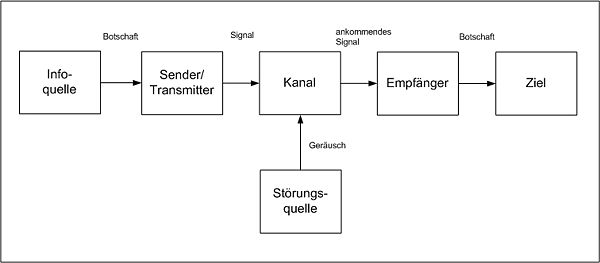
\includegraphics[width=0.6\textwidth]{abb/shannon-weaver-modell.jpg}
	\caption{Shannon-Weaver-Modell}
	\label{fig:shannon-weaver-modell}
\end{figure}

Dieses Modell verdeutlicht zunächst, dass an der Kommunikation stets zwei Instanzen beteiligt sind (Informationsquelle und Ziel).
Die Informationsquelle erzeugt dabei eine Botschaft, welche für das Ziel bestimmt ist und von diesem interpretiert wird.
Diese Kommunikationspartner Senden bzw. Empfangen mittels entsprechender Apparate, welche die zu sendende Botschaft in Signale umwandelt (und umgekehrt).
Meist finden sich diese \ugspr{Geräte} direkt in der Informationsquelle bzw. im Ziel integriert wieder (bei zwischenmenschlicher Kommunikation sind dies Mund und Ohren).
Dieser Informationsaustausch geht immer über einen Kommunikationskanal (z.B. Kabel, Luft, Telefon oder E-Mail). Das darin übertragene Signal kann von Störquellen verfremdet werden.
Kommunikation zeichnet sich in fast allen Fällen zudem durch einen bidirektionalen und wechselseitigen Informationsaustausch aus, d.h. jeder Sender ist gleichzeitig auch Empfänger von Botschaften.
Werden über diesen Weg zwei oder mehr Botschaften ausgetauscht spricht man von einer \fachwort{Interaktion} \citep{human-hacking}.

Um dieses allgemeine Modell für den praktischen Gebrauch nützlich zu machen, gilt es die relevanten Kommunikationskanäle zu definieren und näher zu studieren.
\name{Paul Watzlawick} hat auf diesem Gebiet einige wertvolle Erkenntnisse gewonnen und die fünf \fachwort{pragmatischen Axiome der Kommunikation} formuliert \citep{grundlagen-der-kommunikation}.
Das erste und gleichzeitig Wichtigste dieser Axiome lautet \speech{man kann nicht nicht kommunizieren} \citep[S. 53]{watzlawick}.
\name{Watzlawick} setzt dabei Verhalten der Kommunikation gleich und da es keinen Gegensatz zu Verhalten gibt, ist es auch nicht möglich kein Verhalten zu zeigen ergo nicht zu kommunizieren.
Somit hat jede Art von Verhalten, sofern sie über einen Übertragungskanal vermittelt wird, potenziell einen kommunikativen Charakter.
Ferner hat nach \name{Watzlawick} Verhalten Mitteilungscharakter; somit sind Verhalten und Mitteilung nicht voneinander zu trennen und sollten für ein glaubwürdiges Auftreten kongruent sein.
Diese Aspekte werden vor allem durch den Begriff \fachwort{nonverbale Kommunikation} geprägt.
In Abschnitt \Kapitel{sec:nonverbale-kommunikation} wird detaillierter auf diese Art der Kommunikation eingegangen \citep{grundlagen-der-kommunikation}.
Ein weiteres von \name{Watzlawick} formuliertes Axiom besagt, dass \speech{die Natur einer Beziehung durch die Interpunktion der Kommunikationsabläufe seitens der Partner bedingt} \citep[S. 61]{watzlawick} ist.
Diese Interpunktion von Ereignisfolgen kann mit der Klammersetzung eines mathematischen Terms verglichen werden.
Durch unterschiedliche Positionierung der Klammern (d.h. durch unterschiedliche Interpunktion) entstehen verschiedene Ergebnisse.
Im Bezug auf die Interaktion werden bei kommunikativen Abläufen somit Ursache und Wirkung markiert.
Abbildung \ref{fig:interpunktion} zeigt beispielhaft wie durch Interpunktion Kausalzusammenhänge definiert werden.
Durch das Zurückziehen des Ehemanns beginnt die Frau zu nörgeln, was wiederum das Verhalten des Ehemanns hervorruft.
Gerade in diesem Beispiel ist die Kenntnis über die Interpunktion wichtig, denn genauso ist das Zurückziehen des Ehemanns nur eine Reaktion auf das nörgeln der Ehefrau \citep{grundlagen-der-kommunikation}.
\begin{figure}[htbp]
	\centering
	\includegraphics[width=0.6\textwidth]{abb/Interpunktion.jpg}
	\caption{Interpunktion}
	\label{fig:interpunktion}
\end{figure}

Außerdem unterscheidet eines der in \citep[S. 56]{watzlawick} aufgeführten Axiome zwischen \fachwort{digitaler} und \fachwort{analoger Kommunikation}. Damit sind zwei Ebenen gemeint.
Die digitale Ebene beschreibt die zur Kommunikation verwendeten Worte einer Sprache.
Diese sind dadurch digital, dass ein bestimmtes Wort einer bestimmten Buchstabenfolge entspricht.
Interessanter ist jedoch die analoge Kommunikationsebene.
Darunter fallen sog. \fachwort{paraverbale}, \fachwort{extraverbale} und \fachwort{nonverbale} Sprachanteile \citep{grundlagen-der-kommunikation}.
Diese drei Aspekte werden in Kapitel \KapitelAndName{sec:nonverbale-kommunikation} gemeinsam beschrieben.
Hinzu kommt ein weiteres Axiom, welches eine Aussage über den Beziehungs- und den Inhaltsaspekt \citep{watzlawick} der Nachrichten trifft.
\name{Watzlawick} beschreibt den Zusammenhang dieser zwei Aspekte insofern, dass der Beziehungsaspekt den Inhaltsaspekt beeinflusst und es sich somit um eine \fachwort{Metakommunikation} handelt.
Diese Metainformation gibt dem Empfänger Aufschluss darüber, wie die eigentliche Information zu interpretieren ist.
Ausdrücklich formuliert wird dieser Beziehungsaspekt der Nachricht jedoch nur in den seltensten Fällen \citep{grundlagen-der-kommunikation}.
Das letzte von \citep[S. 50ff]{watzlawick} formulierte Axiom unterteilt Interaktionen in \fachwort{symmetrische} und \fachwort{komplementäre} Interaktionen.
Symmetrische Interaktionen zeichnen sich durch die Gleichheit beider Parteien aus.
Die komplementäre Interaktionen hingegen basiert auf solchen Unterschieden.
Bei dieser Art der Interaktion nimmt eine der Parteien eine übergeordnete Position ein (primäre Stellung), die andere befindet sich in der untergeordneten Position (sekundäre Stellung).
Die übergeordnete Partei, welche die Art der Kommunikation bestimmt, ist dabei aktiv, während die Person in der untergeordneten Position lediglich akzeptiert (passiv) \citep{grundlagen-der-kommunikation}.


\subsubsection{Berlos SMCR-Modell}

Diese von \name{Watzlawick} genannten Axiome bilden eine gute Grundlage für erfolgreiches Social Engineering.
Jedoch sind diese Axiome selbst nur schwer auf konkrete Situationen übertragbar.
Aus diesem Grund bietet es sich an, sich verschiedenerer darauf aufbauender Modelle zu bedienen.
In diesem Abschnitt wird dafür exemplarisch das SMCR-Modell von \name{David Berlo} vorgestellt.
In der Einleitung des Kapitels \nameref{sec:kommunikation} wurde das Kommunikationsmodell nach \name{Shannon} und \name{Weaver} erwähnt.
Dieses sehr allgemeine und eher technisch anmutende Modell wurde 1960 von \name{David Berlo} um einige Aspekte erweitert.
Wie in Abbildung \ref{fig:smcr-model-berlo} zu sehen ist, werden die Hauptkategorien Quelle, Botschaft, Kanal und Empfänger wiederum konkreter definiert.

\begin{figure}[htbp]
	\centering
	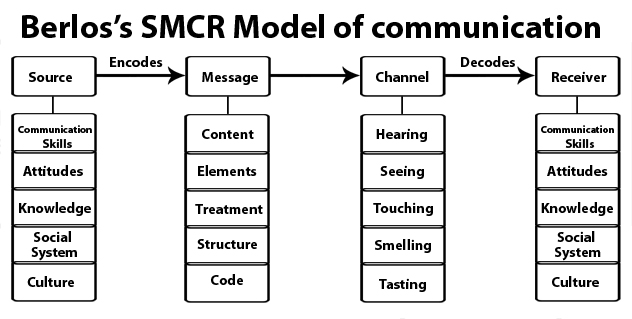
\includegraphics[width=0.6\textwidth]{abb/berlos-smcr-model.jpg}
	\caption{SMCR-Modell von Berlo}
	\label{fig:smcr-model-berlo}
\end{figure}

Bei Sender und Empfänger werden verschiedene individuelle Faktoren berücksichtigt wie z.B. Kultur, Wissen oder die eigenen Kommunikationskenntnisse.
Auch die übermittelte Nachricht wird anhand verschiedener Merkmale analysiert.
Wichtig ist jedoch vor allem die Einordnungsmöglichkeit der Kommunikationskanäle, welche über das Vorhandensein der fünf Sinne ermöglicht wird (Sehen, Hören, Fühlen, Geruchs- und Geschmackssinn).
Abhängig vom gewählten Kanal fallen somit manche dieser Merkmale weg.
Bspw. werden bei einer Videokonferrenz nur die beiden Merkmale Sehen und Hören berücksichtigt.
Bei einer E-Mail wird der Kommunikationskanal zusätzlich auf lediglich das Sehen eingeengt bzw. bei einem gewöhnlichen Telefonat auf das Hören beschränkt \citep{human-hacking}.
Für einen Social Engineer sind dies wichtige Vorüberlegungen, denn die Aufmerksamkeit wird auf nur ein Merkmal der Botschaft verengt, sodass eine tiefere Verarbeitung derselben erfolgen kann.
Dadurch fallen selbst kleinste Fehler leicht auf.
Auch \name{Christopher Hadnagy} nutzt dieses Modell und erweitert es noch durch die Komponente \fachwort{Feedback}, was die vom Angreifer erwartete Antwort im Falle einer korrekten Durchführung darstellt \citep{human-hacking}.

\subsubsection{Nonverbale Kommunikation}\label{sec:nonverbale-kommunikation}

Die Nonverbale Kommunikation ist einer der wichtigsten Kommunikationskanäle.
Schätzungen einiger Experten zufolge macht die Nonverbale Kommunikation ca. 55\% des gesamten Informationsgehalts einer persönlich übermittelten Nachricht aus \citep[S. 4]{tu-dresden}.
Dementsprechend ist die Deutung der Informationen dieses Kanals entsprechend komplex, denn zur Nonverbalen Kommunikation zählen alle körperlichen Gesten, Bewegungen und Haltungen sowie auch akustische Eigenschaften, d.h. neben dem tatsächlich Gesagten, wird der Art wie etwas gesagt wird, ebenfalls eine Bedeutung zugewiesen \citep{hadnagy}.

Im einleitenden Abschnitt \nameref{sec:definition} war bereits die Rede von den durch \name{Watzlawick} definierten Axiomen der Kommunikation.
Dabei wird insbesondere auf sog. \fachwort{Analoge Kommunikation} eingegangen, die \fachwort{extraverbalen}, \fachwort{paraverbalen} und \fachwort{nonverbalen} Eigenschaften.
Als extraverbale Spracheigenschaften bezeichnet man individuelle Stimmeigenschaften, geschlechts- oder altersbedingte Eigenschaften sowie Dialekte und Akzente.
Aus diesen lassen sich bereits Rückschlüsse auf die sprechende Person liefern, da sie jedoch im Laufe einer Kommunikation im Allgemeinen nicht variieren, werden sie hier außen vor gelassen \citep{grundlagen-der-kommunikation}.
Interessanter sind die paraverbalen Sprecheigenschaften, zu denen Merkmale wie Lautheit, Tonhöhe, Sprechgeschwindigkeit und Sprachmelodie gehören.
Diese Eigenschaften sind im englischsprachigen Raum auch durch RSVP abgekürzt (rythm, speed, volume, pitch).
Über bestimmte Ausprägungen dieser Merkmale werden zu dem Gesprochen hinzu weitere Botschaften übermittelt.
So kann eine laute Stimme die Wut über den Gesprächspartner vermitteln, schnelles Sprechen mit hoher Stimme kann ein Zeichen von Unsicherheit sein und lange Pausen können signalisieren, dass der Sprecher nicht die Wahrheit spricht.
Besonders wichtig ist hierbei das Wort \ugspr{kann}.
Die Bedeutung ist grundsätzlich situations- und personenabhängig \citep{grundlagen-der-kommunikation}.
Die mitunter entscheidendsten Eigenschaften sind die eigentlichen nonverbalen Merkmale.
Diese können in die Kategorien Mimik, Gestik und Körperhaltung unterteilt werden.
Aus der Körperhaltung (z.B. Fußstellungen oder Armhaltungen) kann man den Status zwischenmenschlicher Beziehungen während einer Unterhaltung ableiten.
Verschiedene Gesichtsausdrücke lassen außerdem eine solide Einordnung von Gefühlszuständen zu.
Auch aus Arm- oder Handbewegungen können Rückschlüsse auf eine Person und ihren aktuellen Gefühlszustand gezogen werden.
An dieser Stelle sei ein weiteres Mal betont, dass diese Merkmale nicht immer eine Bedeutung haben.
Auch hier können bestimmte Merkmalsausprägungen zur \fachwort{Baseline} der Person gehören und somit keine konkreten Aussagen zulassen \citep{grundlagen-der-kommunikation}.

Abschließend sei erwähnt, dass das Wissen über die nonverbale Kommunikation nicht nur zum Erkennen von Gefühlszuständen genutzt werden kann.
Durch bewusste Kontrolle des Körpers oder der Stimme können gewünschte Stimmungen erzeugt werden.
Dieses Können ist vor allem für den Aufbau eines Vertrauensverhältnisses nützlich.
Weiß man solche Zeichen zu interpretieren und umzusetzen, ist es ein leichtes mittels \ugspr{mirror and match} ein Vertrauensverhältnis aufzubauen \citep{hadnagy}.

\subsection{Instrumente der Manipulation}\label{sec:instrumente_der_manipulation}

Bei Social Engineering geht es wie eingangs in \Kapitel{sec:social_engineering} bereits erwähnt vordergründig nicht darum, den Zugriff auf sensible Daten durch gezielte technische Angriffe gewährt zu bekommen.
Vielmehr geht es darum andere Personen, welche für den Zugriff auf die gewünschten Informationen berechtigt sind, dahingehend zu beeinflussen, Aktionen durchzuführen, die dem Angreifer entweder diese Daten zuspielen oder ihn sogar selbst dafür autorisieren.
Für solche Angriffe bieten sich einige bewährte Methoden an, wie sie unter anderem auch in der Werbebranche
Verwendung finden.
Dabei wird auf verschiedene Mechanismen und Automatismen des menschlichen Verhaltens abgezielt, wie sie ab \Kapitel{sec:reziprozität} erläutert werden sollen.
Es wird dafür in jedem der folgenden Abschnitte eine kurze Erklärung des Prinzips gegeben sowie die Art und
Intensität der Wirkung aufgezeigt und eine Angriffsmöglichkeit im Social Engineering erläutert.
Diese Mechanismen liegen zunächst alle dem Prinzip der Automatismen zugrunde, welches in folgenden Kapitel beschrieben wird.

\subsubsection{Automatismen}\label{sec:automatismen}
In der Psychologie versteht man unter einem Automatismus eine vom Bewusstsein kaum oder gar nicht kontrolliert ablaufende Tätigkeit \citep{duden}.
Bei Lebewesen handelt es sich dabei um fest verankerte Verhaltensmuster.
Entwickelt haben sich diese Mechanismen im Laufe der Evolution und sind somit ein fester Bestandteil der Psyche aller Lebewesen.
Diese Automatismen bestehen im Wesentlichen aus zwei Teilen.
Zunächst ist ein bestimmtes Ereignis nötig.
Dabei kann es sich um einfache Reize aller Art handeln (visuell, akustisch, haptisch, etc.) oder auch um ein komplexes Zusammenspiel mehrerer solcher Reize.
Dieses Ereignis kann leicht eine fest zugeordnete Reaktion triggern, welche den zweiten Teil des Automatismus darstellt.
\citep{cialdini} führt dafür das Beispiel einer Truthenne an.
Diese reagiert auf ein bestimmtes Geräusch, welches ihre Küken von sich geben (akustischer Reiz) damit, dass sie ihre Küken füttert.
Auf den ersten Blick ist dieser Automatismus auch wirksam und hilfreich, denn er erlaubt das herausfiltern relevanter Informationen.
Zwar erspart sich die Henne eine aufwändige Betrachtung der gesamten Informationen, jedoch ist sie dadurch bereits anfällig für eine Art Social Engineering, da Teil, die auf einen Täuschungsversuch hindeuten, können übersehen werden.
Legt man der Henne einen Lautsprecher vor, der eben diese Geräusche von sich gibt, wird sie das gleiche Verhalten zeigen, als würde es sich um ein echtes Küken handeln.

Diese Verhaltensweisen sind bei Tieren zwar besonders stark ausgeprägt, machen allerdings bei uns Menschen nicht gänzlich halt.
Denn auch Menschen benötigten in der Vergangenheit solche Automatismen um zu überleben und benötigen diese auch heute noch, für eine eingehende Betrachtung aller Informationen reicht die Gedächtniskapazität nicht aus.
Der Unterschied zu den Tieren besteht allerdings darin, dass es Menschen leichter fällt diese Automatismen abzulegen.
Nichtsdestoweniger bieten Automatismen auch beim Menschen Potenzial für Social Engineering Angriffe.
In Anbetracht dessen ist es in der Praxis vielmehr das Zusammenspiel vieler Faktoren, die bestimmte Verhaltensweisen auslösen. Konkret sind damit Verhaltensmuster gemeint, welche erst durch die Bildung von Gemeinschaften entstanden sind. Dabei handelt es sich um erlernte Automatismen, die uns den Umgang mit Mitmenschen erleichtern. Aber auch diese Automatismen können ausgenutzt werden, um ein gewünschtes Verhalten auszulösen \citep{cialdini}.


\subsubsection{Reziprozität}\label{sec:reziprozität}
Reziprozität leitet sich vom lateinischen Wort \fremdwort{reziprocus} ab, was mit \translation{wechselseitig} zu übersetzen ist.
Die Wechselseitigkeit tritt dergestalt auf, dass durch Leitungen, Gefälligkeiten o.ä. beim Empfänger derselben das Gefühl entsteht, sich dafür revanchieren zu wollen.
Die Nützlichkeit dieses Mechanismus ist nicht bestreitbar.
So ist es für uns selbstverständlich Dienstleistungen finanziell zu entlohnen, was für eine funktionierende Gesellschaft, wie wir sie kennen, unabdingbar ist.
Das Gleiche gilt für Gefälligkeiten, welche nicht finanziell vergütet werden. Ein Beispiel hierfür ist es, das Anliegen eines Arbeitskollegen bevorzugt zu behandeln. Dadurch dass der anderen Person ein Gefallen erwiesen wird, entsteht bei ihr das Gefühl sich revanchieren zu wollen.
Dieses Phänomen tritt in vielen verschiedenen Variationen auf, welche meist auf einer zuvorkommenden Handlungsweise, einer Art Präsent oder auch einem eigenen Zugeständnis beruhen. Die Intensität der Auswirkung, die das Prinzip der Reziprozität mit sich bringt, hängt in jedem Fall vom Wert der erwiesenen Gefälligkeit bzw. des erbrachten Geschenks ab.
Die bis hierhin beschriebenen Fakten lösen jedoch noch längst keinen Alarm aus, da sie uns Menschen in den meisten Fällen als logische Konsequenz erscheinen.
Allerdings kann Reziprozität auch gegen die Interessen eines Menschen genutzt werden.
Eine Vielzahl von Verkäufern machen sich die Macht der Reziprozität zu Nutze.
Dabei wird bspw. mit einem kleinen Geschenk in Form eines \ugspr{Kennenlernpakets} o.ä. der potenzielle Kunde dahingehend beeinflusst, einem späteren Kaufangebot zuzusagen, da er \ugspr{in der Schuld} des Verkäufers steht \citep{cialdini}.

Dieses Szenario ist nur ein Beispiel von vielen. Grundsätzlich ist jedoch zu erkennen, dass das Ausnutzen der Reziprozität immer das Ziel hat, bestimmte Handlungen beim Opfer auszulösen. Im Kontext des Social Engineering kann dies die Preisgabe kritischer Daten sein. Wie bei einem im vorigen Kapitel beschriebenen Automatismus, liegt die Gefahr der Reziprozität darin, dass Menschen im täglichen gesellschaftlichen Leben darauf angewiesen sind und demnach von ihrer Korrektheit überzeugt sind.

\subsubsection{Konsistenz}

Der Begriff \fachwort{Konsistenz} bezieht sich im Kontext der Soziologie auf den logischen Zusammenhang von Worten, Meinungen und Taten einer Person.
Menschen haben gesellschaftsbedingt das Bedürfnis in dem was sie tun, sagen und glauben konsistent zu sein.
Der Grund dafür liegt darin, dass in unserer Gesellschaft ein hohes Ansehen genießt, wer erlässlich und grundsatztreu handelt.
Menschen, die regelmäßig ihre Meinung ändern, gelten gemeinhin als unberechenbar und nicht vertrauenswürdig.
Persönliche Konsistenz stellt zudem auch in der täglichen Entscheidungsfindung ein verlässliches Werkzeug dar.
So lassen sich mit überschaubarem zeitlichen Aufwand Entscheidungen treffen.
Die Zeitersparnis ergibt sich daraus, dass nicht mehr alle relevanten Informationen überprüft werden und genau an dieser Stelle liegt die Gefahr einer bedingungslos konsistenten oder auch konsequenten Handlungsweise. Diese können auch dazu genutzt werden, bestimmte Aktionen einer Person zu erzwingen \citep{cialdini}.

Ein bekannter Überzeugungstrick ist es, die Zielperson zu einem Statement zu bringen. Durch diese Aussage nimmt sie eine Position ein. Das Prinzip der Konsistenz führt nun dazu, dass diese Person in folgenden Handlungen durch dieses Statement beeinflusst wird. Davon hängt letztlich auch ab, ob die Zielperson der Bitte des Angreifers nachkommt. Dabei ist das folgende Szenario vorstellbar:

Der Angreifer nähert sich einem Rezeptionisten in einem Krankenhaus, um Informationen (Zimmer, Zustand, etc.) über einen Patienten zu erhalten.
Das Gespräch könnte wie folgt ablaufen:

\actor{Angreifer: } \says{Guten Tag. Sie scheinen sehr gut darin zu sein, Leuten zu helfen.}
\actor{Rezeptionist: }\says{Ja, das ist mein Job.}
\actor{Angreifer: }\says{Wären Sie dann so freundlich und sagen mir in welchem Zimmer sich Patient XY aufählt?}
\actor{Rezeptionist: }\says{Natürlich. Patient XY liegt in Zimmer 4711.}

So oder so ähnlich kann sich ein solches Gespräch abspielen. Natürlich hängt der Erfolg eines Manövers dieser Art auch stark von den schauspielerischen Fähigkeiten des Angreifers ab, ob eine solche Aktion glückt.
Die Essenz dieses Angriffs ist und bleibt jedoch das Konsistenz-Prinzip. Der Rezeptionist macht hierbei eine Aussage über seine Fähigkeit Menschen eine gewünschte Auskunft zu geben. Das Nicht-Preisgeben der Information würde demnach gegen das Konsistenz-Bewusstsein der Zielperson verstoßen. Wie stark dieses Bewusstsein ist, hängt wie im vorigen Kapitel zur Reziprozität beschrieben ebenfalls von der vorangegangenen Handlung ab. In diesem Fall handelt es sich dabei um die Intensität des gemachten Statements.

Faktoren, die die Auswirkungen eines solchen Statements verstärken, sind Aktivität des Opfers (wird das Statement selbst formuliert oder lediglich bestätigt?), Öffentlichkeit (hören andere Leute zu?) und auch die Ungezwungenheit (hat das Opfer das Gefühl zu einem Statement gedrängt worden zu sein?) \citep{cialdini}.
Anders als im bereits aufgeführten Beispiel, kann auch eine genaue Analyse der Zielperson Angriffspunkte offenlegen.

\subsubsection{Sympathie}\label{sec:sympathie}
Die in den vorangegangenen Kapiteln beschriebenen Mechanismen lassen sich auch mit anderen \ugspr{Techniken} kombinieren. Es ist allgemein bekannt, dass es besonders solchen Menschen leicht fällt uns zu Manipulieren, welche uns sympathisch sind.
Sympathie wirkt wie ein sozialer Katalysator bei der Überzeugung anderer Menschen. 
An dieser Stelle soll zunächst erläutert werden, wie Sympathie entsteht und von welchen Faktoren sie abhängt.

Das ausschlaggebendste Kriterium, welches beeinflusst, ob wir eine Person sympathisch finden, ist tatsächlich die körperliche Attraktivität. Besonders bei gut aussehenden Menschen ist der sogenannte \fremdwort{Halo-Effekt} zu beobachten (dt. Heiligenschein-Effekt). Menschen schließen von der äußerlichen Schönheit einer Person direkt auf andere (davon unabhängige) Eigenschaften wie z.B. Kompetenz, Freundlichkeit
oder Begabung.
Neben körperlicher Attraktivität ist auch die Ähnlichkeit zur Zielperson selbst ausschlaggebend. Hierbei spielen sowohl äußerliche sowie charakterliche Merkmale und auch Ansichten eine wichtige Rolle.
Sympathie kann zudem durch die wiederholte Kontaktaufnahme mit der Zielperson aufgebaut werden. Dabei ist es umso förderlicher, wenn mit dem Kontakt eine erfolgreiche Kooperation einhergeht (welcher Art auch immer). Verstärken lässt sich der Effekt auch durch das Erteilen von Komplimenten. Denn durch das Erhalten eines Kompliments tritt zusätzlich der Effekt der Reziprozität in Kraft. Bei einem Kompliment handelt es um eine Art Geschenk, welches es zu erwidern gilt. So äußert die Zielperson bspw., dass sie eine bestimmte Eigenschaft der Person gegenüber schätzt. Somit ist außerdem ein Statement geäußert (\speech{Mein Gegenüber ist nett}), was das Konsistenz-Bewusstsein anspricht \citep{cialdini}.

Die Sympathie ist demnach bestens dafür geeignet mit anderen manipulativen Werkzeugen eingesetzt zu werden, da sie die Willfährigkeit anderer Menschen verstärkt. Die Sympathie ist gerade deshalb gefährlich, weil sie dem Menschen im Alltag ein bekannter jedoch oberflächlicher Ratgeber ist, welchen Personen man trauen kann bzw. welche man besser meidet.

\subsubsection{Autorität und Befehle}\label{sec:autorität-und-befehle}
Eine gegensätzliche und dennoch überraschend ähnliche Methode Menschen zu überzeugen ist die Macht der Autorität.
In unserer Gesellschaft besteht ein starker Druck, was das befolgen von Anweisungen durch eine Autorität betrifft.
Damit sind zunächst einmal nur echte Autoritäten gemeint.
Gefährlich wird es, sobald Meinungen oder Befehle einer Autorität nur noch hingenommen und nicht mehr hinterfragt werden.
Denn hinter solchen Befehlen kann sich ein Fehler verbergen oder eine falsche Autorität in Form eines Social Engineers.
Es ist aus diesem Grund wichtig zu wissen, wann eine bestimmte Person für eine Autorität bzw. einen Experten gehalten wird. Meist wird nicht die eigentliche Autorität wahrgenommen sondern nur Symbole, die auf eine solche hindeuten. Bei solchen Symbolen handelt es sich im Speziellen um Kleidung (Arztkittel, Uniform, usw.), auch um Titel (Graf, Prof., Dr. med., etc.) oder andere äußerliche Merkmale wie die Körpergröße  \citep{cialdini}.
Die Autoritätshörigkeit, wie wir sie kennen, ist deshalb so oft vorzufinden, da Menschen unserer Gesellschaft darauf gedrillt werden Anweisungen von Autoritäten zu folgen, da diese über mehr Wissen, Macht oder Erfahrung verfügen. Zusätzlich werden Autoritäten auch zur Vereinfachung der eigenen Entscheidungsfindung herangezogen \citep{hacking-the-human}.

\section{Risikoanalyse und -management}\label{sec:risikoanalyse}
In den vorigen Kapiteln ist das Prinzip von Social Engineering erläutert worden und somit aufgezeigt
geworden, wie leicht solche Angriffe von statten gehen können und welche Gefahren im Vergleich zu
herkömmlichen Angriffsmethoden bestehen.
Dennoch wird das von Social Engineering herrührende Risiko oft unterschätzt.
Um diesen Gefahren zielgerichtet entgegenzuwirken, ist es wichtig ein grundlegendes, allgemeines
Verständnis von Risikofaktoren, deren Bewertungen und Handhabung zu bekommen.
Dieses Kapitel vermittelt zunächst, wobei es sich bei dem Begriff Risiko im Allgemeinen handelt.
Es wird außerdem geschildert, aus welchen Gründen meist kein angemessenes Risikomanagement
zur Anwendung kommt.
Abschließend werden diese allgemeinen Erkenntnisse auf den Bereich der speziellen Risikofaktoren durch
Social Engineering Angriffe übertragen (s. \Kapitel{sec:social_engineering_als_risikofaktor}).

\subsection{Risiken}\label{sec:allgemeines}
Risiken im Allgemeinen und ihre Handhabung treten in nahezu allen Situationen des täglichen Lebens
auf.
Dabei kann es sich um solche trivialer Natur handeln wie der Wahl eines Getränks bis hin
zur Entscheidung für oder gegen die Investition in eine Aktie.
Auch wenn beide Situationen sehr unterschiedlich anmuten, haben sie sehr viel gemeinsam.
Sowohl die Wahl eines Getränks als auch die Investition in eine Aktie bergen ein gewisses Risiko.
Offensichtlich bieten die beiden Aktionen unterschiedlich große Risiken, weswegen es notwendig ist,
solche Risiken korrekt einzustufen und zu bewerten.
Ein wichtiges Merkmal für ein Risiko ist, dass eine jede Entscheidung mit einem Risiko verknüpft ist,
wobei es sich dabei auch um die Entscheidung nichts zu tun handeln kann.
In Bezug auf Informationssicherheit kann eine Gefahr bedeuten, dass geschäftskritische Daten für
nicht-autorisierte Nutzer zugänglich gemacht werden.
Trifft man in einem solchen Fall die Entscheidung nichts zu tun, ist das damit verbundene Risiko der Offenlegung kritischer Informationen entsprechend hoch.
Die Auseinandersetzung mit Entscheidungen, den damit Verbunden Risiken und den Möglichkeiten des
zweckmäßigen Umgangs ist vor allem wertvoll für die positive Beeinflussung zukünftiger Situationen.
Die Analyse von Risiken sollte nicht dazu verwendet werden Ereignisse zu erklären welche der
Vergangenheit angehören.

In Bezug auf den Umgang mit Risiken gibt es verschiedene Herangehensweisen, welche nicht in der Reinform auftreten, generell jedoch oft wiederzuerkennen sind.
Die \fachwort{fatalistische} Herangehensweise zeichnet sich besonders durch die damit verbundene Passivität aus.
Dabei wird davon ausgegangen, dass zukünftige Ereignisse weder abwendbar noch voraussehbar sind.
Auffällig ist, dass das Handeln ausschließlich aus Reaktionen besteht.
Ein anderes Extrem ist der \fachwort{fanatische} Ansatz.
Hierbei wird von einer konkreten Zukunft ausgegangen, welche man in diesem Zusammenhang als Vision bezeichnen kann.
Abweichungen von dieser Vision in Form anderer Möglichkeiten werden gänzlich ignoriert und lösen auch
keine notwendigen Reaktionen aus.
Dass diese beiden Handlungsweisen nicht zielführend sind, ist offensichtlich.
Allerdings ist auch eine rein wissenschaftliche Beurteilung von Risikosituationen nicht von Nutzen.
Ein rein wissenschaftlicher Ansatz ist zwar unvoreingenommen, zeichnet sich jedoch durch die
Notwendigkeit einer stichhaltigen Beweislage aus.
Da diese für in der Zukunft liegende Ereignisse nicht vorhanden ist, würde der rein wissenschaftliche
Ansatz nie zu einer endgültigen Entscheidung führen.
Der \fachwort{pragmatische} Ansatz geht von der Annahme aus, dass die Zukunft zwar ungewiss ist, allerdings nicht gänzlich unvorhersehbar ist.
Dabei sollen die Chancen positiv verändert werden, während eine mangelnde Beweislage akzeptiert wird \citep{risikomanagement}.

\subsection{Risikomanagement}\label{sec:risikomanagement}
Der Umgang mit Risiken setzt sich aus mehreren Schritten zusammen.
Der erste und wichtigste Schritt ist die Identifizierung von Risiken.
Die Schwierigkeit besteht im Grunde darin, dass nicht klar ist, wonach überhaupt gesucht wird.
Das liegt an der bislang noch spärlichen Kategorisierung von Risiken.
In der Informationssicherheit sind jedoch viele Risiken bereits bekannt, obgleich sich die Methoden
schnell weiterentwickeln.
Ein Risiko stellt auch die Bedrohung durch Social Engineering Angriffe dar.
\citep{risikomanagement} empfiehlt beim Umgang mit Risiken verschiedene Taktiken.
Dabei wird beispielsweise die Vermeidung und Verteilen der Risiken vorgeschlagen.
Im Falle von gespeicherten Informationen stellen diese Lösungsansätze allerdings keine brauchbaren
Alternativen dar.
Zwei Möglichkeiten für den Umgang mit Risiken solcher Art sind zum einen die Versicherung für den
Fall, dass ein Schadensfall eintritt, zum anderen die gezielte Absicherung.
Da mit dem Verlust solcher Daten an Dritte nicht nur finanzieller Schaden sondern auch ein immenser
Imageschaden einhergeht, ist auch die Herangehensweise mit einer Versicherung nicht zweckgemäß.
In aller Regel bildet nur ein gezielter Schutz vor Angriffen eine angemessene Art des
Risikomanagements.

\subsection{Ursachen für schlechtes Risikomanagement}\label{sec:ursachen}
Oft stehen dem korrekten Umgang mit Risiken allerdings einige Hürden im Weg.
Zum einen sind es sicherlich Schätzungen und Vereinfachungen, die eine Fehlerquelle bilden.
Viel gefährlicher sind jedoch Fehlerquellen menschlicher Natur.
Diese Hindernisse zur rationalen Entscheidungsfindung gründen auf grundlegenden Eigenschaften der menschlichen Psyche (welche wiederum die Grundlage für die Techniken des Social Engineering bildet).
Menschen neigen häufig dazu die eigenen Möglichkeiten zu überschätzen.
Möglichkeiten, denen eine sehr geringe Wahrscheinlichkeit zugeordnet ist, werden oft ausgeblendet und
als unmöglich bezeichnet.
Die Tendenz bei Menschen geht allerdings dahin, dass dies stärker bei Risiken geschieht, als bei der
Wahrnehmung von Möglichkeiten \citep{risikomanagement}.
Die Ursache hierfür ist das Phänomen des menschlichen Optimismus.
Negative Resultate werden vielmals unterschätzt und unverhältnismäßig hohe Risiken werden für Chancen
mit geringer Aussicht auf Erfolg aufgenommen.

Zum anderen ist oft eine fälschliche Betrachtung vergangener Ereignisse zu beobachten.
Im Detail bedeutet das, dass eingetretenen Ereignissen der Vergangenheit im Nachhinein nachgesagt
wird, sie seien absehbar gewesen, auch wenn sie vor ihrem Eintreten als unwahrscheinlich eingeordnet
worden sind.
Mit dieser rückblickenden Betrachtung werden aus optimistischen Herangehensweise resultierende
Fehlentscheidungen gerechtfertigt und beschönigt \citep{risikomanagement}.

Vielen Menschen fällt es außerdem schwer an die Beliebigkeit und die Zufälligkeit von Ereignissen zu
glauben.
Tatsächlich neigen sie dazu nach Mustern zu suchen und Ereignisse in eine Ordnung zu bringen.
So werden beispielsweise aus einer Entwicklung über eine relativ kurze Zeit Rückschlüsse für die Zukunft geschlossen.
Ähnlich dem Suchen von Mustern geht die Kurzsichtigkeit bei der Beurteilung von Ereignissen einher.
Dies kann unter anderem bei Fußballtrainern zu beobachten.
Schon eine kurze Serie an Niederlagen, verleitet Fans und Vereinsvorstand die Ursache beim Trainer zu
suchen.
Viele Trainer werden schon nach kurzen Zeiträumen bereits entlassen, ohne dass eine solide
Informationsbasis zur rationalen Entscheidungsfindung existiert hat.
Einen Fußballtrainer nach einer Serie von Niederlagen zu entlassen, ist zwar eine harte
Entscheidungsfindung, aus risikoanalytischen Gesichtspunkten jedoch immer noch sinnvoller als die
Passivität.
Die Ursache hierfür liegt darin, dass Menschen eine falsche Aktion negativer bewerten als das
Unterlassen einer Aktion, auch wenn die Passivität das schlechtere Ergebnis liefert.
Gerade in Bezug auf die Informationssicherheit ist es undenkbar keine Gegenmaßnahmen zu treffen oder
im Falle eines Informationsverlustes in Tatenlosigkeit zu verharren.

Eine Bekannte Ursache für eine Fehleinschätzung von Risiken sind ironischerweise
Sicherheitsmechanismen wie der Sicherheitsgurt im Auto oder ein verbesserter Algorithmus zur
Berechnung des Risikos für Finanzanlagen.
Eben diese risikominimierenden Algorithmen sorgen dafür, dass sich der Anwender in Sicherheit wähnt
und damit in Summe ein größeres Risiko eingeht, als er ohne diese Absicherung eingegangen wäre.

Der letzte signifikante Punkt, welcher von \citep{risikomanagement} erwähnt wird, ist die Selbstzufriedenheit des Menschen. Darunter ist zu verstehen,
dass dem Menschen bekannte Risiken weniger gefährlich erscheinen als solche, die über seine Gewohnheit
hinausgehen.
Gerade in Bezug auf Social Engineering ist dieser Punkt erwähnenswert, denn es ist dem Menschen in der
Tat eine Gewohnheit, mit anderen Menschen zu interagieren.
So fällt es Menschen schwer das Risiko zu erkennen, welches von einem Gespräch ausgehen kann.
Grundsätzliche Skepsis ist allerdings ebenso kontraproduktiv und es muss abgeschätzt werden
inwiefern Sicherheitsvorkehrungen bei internen und externen Gesprächen eines Unternehmens sinnvoll
sind.


\subsection{Risikofaktoren des Social Engineering}\label{sec:social_engineering_als_risikofaktor}
Bis zu diesem Kapitel wurde das Phänomen Social Engineering und die grundlegende Idee dahinter
beschrieben sowie der Umgang mit Risikofaktoren und den Hindernissen der menschlichen Psyche.
Social Engineering bildet unbestreitbar einen beachtenswerten Risikofaktor.
Dabei gibt es eine Vielzahl an möglichen Szenarien, die beobachtet und analysiert werden können.
Leider ist es zu oft der Fall, dass erfolgreiche Angriffe die auf Social Engineering basieren in den
seltensten Fällen als solche identifiziert werden.
Gerade weil Angriffe dieser Art oft in Kombination mit technischen Methoden angewandt werden, wird ein
rein technischer Angriff dokumentiert.
Aus diesem Grund und eines allgemein fahrlässigen Risikomanagements wegen wird in vielen Unternehmen
die Gefahr von Social Engineering nicht angemessen ernst genommen.
Zudem wird der Umgang mit Daten verschiedener Art nicht ausreichend kritisch beleuchtet.
Viele Informationen werden oft fälschlicherweise als nicht-vertraulich eingestuft.
In vielen Unternehmen besteht jedoch genau an diesem Punkt ein großer Irrtum.
Denn aus der Sicht eines Social Engineers gibt es keine irrelevanten Informationen.
Für einen Angreifer sind bereits kleine Details zu einzelnen Mitarbeitern hilfreich; auf der Grundlage des Vor- und Nachnamens lassen sich bereits viele weitere Informationen mittels Internetrecherche herausfinden.
Auch branchen- oder firmeneigene Fachtermini sind für den Social Engineer von Nutzen.
Zwar ist der Schutz vor solchen Auskünften freilich nur schwerlich zu verhindern, jedoch gerät man sehr schnell in eine Grauzone.
Man denke dabei nur an Mitarbeiternummern, Nummer einer Kostenstelle oder ein internes Organigramm.
Solche von den Mitarbeitern für harmlose Daten gehaltenen Informationen, sind für Social Engineering Attacken leicht gefundene Angriffsziele.
Um diese Gefahren einzugrenzen ist es für Unternehmen wichtig den Mitarbeitern die verschiedenen Bedeutungen vermeintlich nicht-vertraulicher Informationen klar zu machen \citep{mitnick2006kunst}.

\section{Umfrage}\label{sec:umfrage}
Bis hierhin ist geschildert worden, worum es sich bei Social Engineering handelt, welche Techniken dabei zum Einsatz kommen und wie das damit verbundene Risiko einzuschätzen ist.
Um die tatsächlichen Anfälligkeiten zu überprüfen ist im Rahmen der Studienarbeit eine Umfrage durchgeführt worden, bei welcher verschiedene berufstätige Personen zu verschiedenen Themen befragt wurden.
Die Umfrage mit dem Titel \ugspr{Hilfsbereitschaft und Social Engineering} und die daraus gewonnenen Ergebnisse werden im folgenden vorgestellt, aufbereitet und diskutiert.
Ebenfalls wird die Vorgehensweise skizziert.

\subsection{Fragebogen}
Für die Verteilung und Erstellung wurde das Web bzw. die Software Limesurvey verwendet.
Die Umfrageergebnisse sind mittels einiger demographischer Daten kategorisiert.
Bei den für diese Umfrage erhobenen Daten handelt es sich um das Alter, das Geschlecht, die Berufsgruppe, die Unternehmensgröße sowie die Anzahl der Standorte.
Im weiteren Verlauf werden Fragen zu verschiedenen Themenschwerpunkten gestellt.
Dabei handelt es sich konkret um Fragen zu Hilfsbereitschaft, Vertrauen, Aufmerksamkeit und einigen abschließenden Fragen zu Social Engineering selbst.

Im ersten Abschnitt (Hilfsbereitschaft) werden Fragen zu Situationen im Arbeitsalltag gestellt.
Diese Szenarien sind maßgeblich an den in Kapitel \ref{sec:gangige_angriffe} vorgestellten Angriffsmustern orientiert und sollen die Anfälligkeit der Probanden nachweisen.
Bei den Fragen handelt es sich um Ja/Nein-Fragen, bei denen angegeben werden soll, ob man dazu tendiert die erwartete Handlung auszuführen oder diese zu unterlassen.
Bei den ersten drei Fragen handelt es sich um direkte Angriffe bei denen eine gesamte Identität vorgetäuscht wird, die letzte Frage bezieht sich auf die Technik Phone Elicitation.
Zudem überprüft die letzte Frage die Mitteilungsbereitschaft gegenüber den anderen Geschlecht.

Die darauf folgende Serie von insgesamt sechs Fragen bezieht sich auf das Vertrauen der Probanden.
Dabei gibt es Fragen zu allen der drei Angriffskategorien: Identitätsbetrug, Phone Elicitation und E-Mail-Phishing.
Dabei wird das Vertrauen in die Identität von angezeigten Telefonnummern und E-Mail-Adressen (und somit indirekt das bewusste Wissen über Spoofing-Techniken) überprüft.
Damit ist die Problematik gemeint, dass eine Person tatsächlich über dieses Thema informiert ist, in der konkreten Situation jedoch nicht daran denkt.
Die letzten beiden Fragen zeigen Bilder von jeweils einer Person und sollen prüfen inwiefern die Optik das Vertrauen beeinflusst.
Innerhalb dieser Serie sollen Bewertungen des Vertrauens auf einer Skala von eins bis fünf angegeben werden.

In der folgenden Kategorie werden dem Probanden drei Bilder gezeigt, welche jeweils verschiedene Personen darstellen.
Zum einen wird eine Reinigungskraft gezeigt, welche gerade einen Fußboden wischt, zum anderen ein Techniker, der gerade an einer Art Verteilerkasten steht sowie eine Führungskraft.
Dabei soll der Proband angeben wie sehr er diese Personen im Arbeitsalltag wahrnimmt.
Wie in der vorangegangen Kategorie wird dies mittels einer Skala von eins bis fünf festgestellt.
Abschließend werden Fragen zu Social Engineering gestellt.
Der Proband wird dabei gefragt, ob er von Techniken wie Spoofing bereits gehört hat.
Außerdem soll er eine persönliche Einschätzung des Risikos abgeben.

Die Umfrage selbst ist für den Zeitraum von ca. sechs Wochen öffentlich verfügbar gewesen und ist von freiwilligen Probanden durchgeführt worden.
Verteilt wurde die Umfrage weitestgehend mittels sozialer Netze.

% Bezüge auf psychologische Grundlagen machen

\subsection{Nachträgliche Betrachtung}
Im Rückblick vor allem jedoch durch die Betrachtung der Ergebnisse sind einige Punkte verdeutlicht worden, welche dem Fragebogen Aussagekraft entziehen bzw. Potenzial für weitere Aussagen entzogen haben.
Innerhalb der demographischen Daten ist es wie den Ergebnissen des Fragebogens zu entnehmen ist, leider nicht gelungen, die Berufsgruppen sinnvoll abzudecken.
Zwar können Kernaussagen darüber getroffen werden, inwiefern sich IT-affine Berufsgruppen von solchen Unterscheiden, die sich nicht näher damit beschäftigen, jedoch ist innerhalb letzterer keine Möglichkeit gegeben genauere Erkenntnisse zu gewinnen.
Eine granulare Aufteilung ist an dieser Stelle sicherlich interessant und würde für verschiedene Bereiche in Unternehmen einen sinnvollen Aufschluss darüber geben, welche Abteilungen leichter anzugreifen sind als andere.
Auch sind andere Merkmale gar nicht erfasst worden wie z.B. die Dauer der Berufstätigkeit oder wie viele verschiedene Berufsgruppen an einem Standort vertreten sind. % Merkmale nennen

Die Fragen, welche Personen zeigen, haben seitens der Auswertung ein großes Potenzial, welches aufgrund der begrenzten Umfragedauer nicht vollständig ausgeschöpft werden konnte.
So könnte man zur Fragegruppe Wahrnehmung wesentlich detailliertere Erkenntnisse gewinnen.
Gerade in Kombination mit genaueren Angaben im Bereich der Berufsgruppe können hierbei sicherlich nützliche Hinweise herausgearbeitet werden.

Alldem ist hinzuzufügen, dass es sich bei den Ergebnissen letztlich nicht um eine Überprüfung des Ernstfalls handelt sondern lediglich eine theoretische Befragung vorliegt.
Unterschiede zu einer Situation wie sie tatsächlich vorkommt liegen vor allem in der persönlichen Distanz der Person.
Wird man auf einem Fragebogen mit einer solchen Situation konfrontiert ist es wesentlich besser möglich sich davon zu distanzieren und klarer darüber nachzudenken.
Zudem ist dem Probanden dadurch mehr Zeit gegeben.
Zwar sind die Probanden zum einen darauf hingewiesen worden, dass es sich um ein anonyme Umfrage handelt, zum anderen wurde darum gebeten die Fragen so zu beantworten, dass es dem eigenen Verhalten entspricht, jedoch ist nicht auszuschließen, dass ein kleiner Anteil der Anworten von der tatsächlichen Handlungsart des Probanden abweichen kann.


% evtl Straßenbefragungen machen??
% Jürgen & Simone?
\subsection{Ergebnisse}

\subsection{Auswertung}
% an dieser Stelle sollten noch einige Schwachstellen des Tests dargelegt werden.

\input{6_hardening}

\section{Diskussion und Ausblick}\label{diskussion-und-ausblick}

Im Verlauf der vorliegenden Arbeit wurde zunächst an das Thema Social Engineering herangeführt und einige grundlegende Angriffsmuster beschrieben.
Die mit solchen Angriffen erreichte Effizienz ist erschreckend und ist ein klares Zeichen für Unternehmen diese Bedrohung ernst zu nehmen.
Vor allem die diffizile forensische Aufklärung solcher Angriffe macht es schwer genaue Zahlen zu erfassen, denn oftmals stehen hinter scheinbar rein technischen Angriffen die Methoden eines Social Engineers am Anfang der Kausalkette.
Zwar ist in sehr großen Konzernen die Gefahr bereits erkannt und korrekt eingeschätzt, jedoch ist es vor allem in kleinen und mittelständischen Unternehmen ein noch nicht ernst genug genommenes Thema.
Hacking Angriffe zielen zwar meist auf militärische Einrichtungen, Banken oder ähnliche Institutionen ab, jedoch liegt das Risiko für andere Branchen bei weitem nicht bei null.
Wie das Kapitel über \nameref{sec:risikoanalyse} gezeigt hat, werden viele Risiken wie Social Engineering oft nicht ernst genug genommen und zu oft darauf gehofft, dass ein negatives Ergebnis ausbleibt.
Gewissenhafte Datenschutzbeauftragte in Firmen sollten demnach überlegen das Unternehmen und seine Mitarbeiter gegen Angriffe dieser Art zu schützen.
Problematisch können an dieser Stelle selbstverständlich die aufkommenden Kosten für eine solide Implementierung von Abwehrmaßnahmen sein.
Es kann jedoch aktiv ein Verständnis der Vertraulichkeit von Daten gelebt werden, was schon mit wenigen Mitteln stark verbessert werden kann.

Die Umfrage bestätigt in einigen Punkten die Dringlichkeit einer intensiveren Aufklärung.
Zwar gaben nur wenige Probanden an einen Mitarbeiter mit defekten/fehlenden ID-Chip einzulassen, jedoch wurde auf Bitten anderer Szenarien weitaus freizügiger reagiert.
Zwar gibt es leichte Schwankungen zwischen Berufsgruppen welche in der EDV angesiedelt sind und anderen Berufsgruppen, diese beziehen sich jedoch größtenteils auf Situationen in denen es konkret um Aktivitäten an IT-Geräten geht.
Wenn es sich um Zugangskontrollen oder ähnliches handelt gleichen sich die Ergebnisse an.
Sicherlich bietet das Grundprinzip solcher Umfragen noch weiteres Potenzial zur genaueren Untersuchung.
Einzelne Zielgruppen können genauer analysiert werden, um somit genauere Vorstellungen von den Schwachstellen aufzudecken.



\section{Fazit}\label{fazit}

\onecolumn
% einfacher Zeilenabstand
\singlespacing
% Literaturliste soll im Inhaltsverzeichnis auftauchen
\newpage
\addcontentsline{toc}{section}{Literaturverzeichnis}
% Literaturverzeichnis anzeigen
\renewcommand\refname{Literaturverzeichnis}
\bibliography{Hauptdatei}

%% Index soll Stichwortverzeichnis heissen
% \newpage
% % Stichwortverzeichnis soll im Inhaltsverzeichnis auftauchen
% \addcontentsline{toc}{section}{Stichwortverzeichnis}
% \renewcommand{\indexname}{Stichwortverzeichnis}
% % Stichwortverzeichnis endgueltig anzeigen
% \printindex

\onehalfspacing
% evtl. Anhang
\newpage
\addcontentsline{toc}{section}{Anhang}
\fancyhead[L]{Anhang} %Kopfzeile links
\subsection*{Anhang}\label{anhang}


% Eidesstattliche Erklärung
\addcontentsline{toc}{section}{Eidesstattliche Erklärung}
\section*{Eidesstattliche Erklärung}
\thispagestyle{empty}

\begin{verbatim}

\end{verbatim}

\begin{LARGE}Eidesstattliche Erklärung zur <-Arbeit>\end{LARGE}
\begin{verbatim}


\end{verbatim}
Ich versichere, die von mir vorgelegte Arbeit selbstständig verfasst zu haben. Alle Stellen, die wörtlich oder sinngemäß aus veröffentlichten oder nicht veröffentlichten Arbeiten anderer entnommen sind, habe ich als entnommen kenntlich gemacht. Sämtliche Quellen und Hilfsmittel, die ich für die Arbeit benutzt habe, sind angegeben. Die Arbeit hat mit gleichem Inhalt bzw. in wesentlichen Teilen noch keiner anderen Prüfungsbehörde vorgelegen.



\begin{displaymath}
% use packages: array
\begin{array}{ll}
Unterschrift:~~~~~~~~~~~~~~~~~~~~~~~~~~~~~~~~~~~~~~~~~~
& Ort, Datum:~~~~~~~~~~~~~~~~~~~~~~~~~~~~~~~~~~~~~~~~~~
\end{array}
\end{displaymath}


% leere Abschlussseite
\newpage
\thispagestyle{empty} % erzeugt Seite ohne Kopf- / Fusszeile
\section*{ }

\end{document}